
\documentclass[sigconf,authordraft]{acmart}

\AtBeginDocument{%
  \providecommand\BibTeX{{%
    \normalfont B\kern-0.5em{\scshape i\kern-0.25em b}\kern-0.8em\TeX}}}
\setcopyright{acmcopyright}
\copyrightyear{2018}
\acmYear{2018}
\acmDOI{10.1145/1122445.1122456}

%% These commands are for a PROCEEDINGS abstract or paper.
\acmConference[Woodstock '18]{Woodstock '18: ACM Symposium on Neural
  Gaze Detection}{June 03--05, 2018}{Woodstock, NY}
\acmBooktitle{Woodstock '18: ACM Symposium on Neural Gaze Detection,
  June 03--05, 2018, Woodstock, NY}
\acmPrice{15.00}
\acmISBN{978-1-4503-XXXX-X/18/06}
\usepackage{natbib}



\usepackage{natbib}
\begin{document}

\title{New York Citi Bike Trip Histories\\
\large Project Proposal\\
EECS 6414 Data Analytics and Visualization}

\author{Sajjad Pakdaman Sovoji}
\affiliation{%
  \institution{York University}
  \streetaddress{4700 Keele Street}
  \city{Toronto}
  \state{Ontario}
  \country{Canada}
  \postcode{M3J1P3}
}
\email{savoji@yorku.ca}

\author{Amin Fadaeinejad}
\affiliation{%
  \institution{York University}
  \streetaddress{4700 Keele Street}
  \city{Toronto}
  \state{Ontario}
  \country{Canada}
  \postcode{M3J1P3}
}
\email{afadaei@yorku.ca}

\author{Pouya (Adrian) Firouzmakan}
\affiliation{%
  \institution{York University}
  \streetaddress{4700 Keele Street}
  \city{Toronto}
  \state{Ontario}
  \country{Canada}
  \postcode{M3J1P3}
}
\email{Adrianfi@yorku.ca}


\begin{abstract}
During the last decade, people all around the world have become considerably fond of environmentally friendly transportation such as public transportation and of course using bicycles to commute. In this regard, this project is up to focus on a number of datasets related to the bike trips history of New York City as one of the largest cities in the world. The contribution of the project would bring about remarkable benefits to the transportation system and its improvement.
\end{abstract}



\keywords{Data Analytics, Data Visualization, Bike Trips History,Bike Stations, New York City}


\maketitle

\section{Motivation and Domain Description}


The concentration of this project is on a set of datasets related to Transportation/City Management  \cite{last.fm} . In this regard, the goal of this project is to perform a detailed analysis of the chosen dataset. Doing so we hope to find viable answers to the questions described in the following sections. Analysis of such a transportation system is important as concluding effective results can help the governing section to effectively maintain this transportation network and improve its coverage and throughput by managing the bike stations in the city of New York. Moreover, due to the fact that this data was collected from a human user-based network, one might use it to extract usage behavior on a personal or social level. The potential questions that are going to be answered are as follow:
\begin{itemize}
    \item Which stations are most commonly used? Is there any spatial/geographical reason for that?
    \item  Are there any usage trends in terms of average trip duration and distance?
    \item During which time spans in a day these bikes are most commonly used?
    \item  Using the number of trips starting and those ending in stations, can we come up with a non-uniform bike allocation scheme?
    \item What are the potential locations for expansion of this network? \href{https://ride.citibikenyc.com/blog/major-citi-bike-expansion-map-revealed}{\color{blue} (link)}
     \item Has the pandemic affected the growth of bike share? And to what extent?\href{https://www.nytimes.com/2021/12/02/nyregion/citi-bike-parking-docking-station.html}{\color{blue} (link)}
     \item Is there a footprint of maintenance routines in the data set?
     \item Does gender have an impact on one's usage pattern?

\end{itemize}

It is worth mentioning that such analysis can be used for governing decisions. These decisions made based on this analysis can dramatically affect the experience of the bike users by improving/decreasing its efficiency and accessibility. With that in mind, such major changes in a transportation system can result in total destruction or growth in the number of users. On the other hand, the applications of this project are specified but not limited to shared transportation systems including bike share, car share, car rental(uber/lyft).






\section{Methodology}


\subsection{Data analytics methods to be employed:} As this project aims to extract meaningful relations from the aforementioned dataset, our methodology expands in several domains. For some tasks/relations the analysis will be limited to simple statistical operations such as pdf estimation(histograms) and statistical exams while for other tasks/relations, it might include machine learning algorithms, most probably as a regressor. Furthermore, many of such spatial relations in the dataset can only be obtained via visual explanations. As such a major part of our methodology will be creating meaningful visualizations from the dataset. \cite{schneider_2015}

\subsection{What are the steps you need to perform:} First the data needs to be preprocessed properly. Some of the columns are not initially ready to be used in data analytics approaches as they do not represent numbers; for example, the address of bike stations and their corresponding coordinates should be translated to the correct format. Once the data is preprocessed, it should be loaded via a secondary platform such as pandas. Next data analytics algorithms should be performed on the loaded data. As mentioned before, depending on the task it might include simple statistical exams or learning a regressor for prediction. In the next stage, the results of those algorithms should be assessed via quantitative and qualitative measures. Last but not least, these results should be visualized via a secondary platform such as Tableau. \cite{rogozhin_2020}

\subsection{Are there any technical problems you need to solve?} One major technical problem that needs to be faced during this project is working with a huge amount of data. This data has been gathered since 2013 which makes it almost 8 years of bike trips in NYC. This dataset is estimated to contain more than 10 million trips recorded, making it probably impossible to be loaded into the main memory of available computing devices. Therefore there is a need to implement most algorithms in a fashion that data can be placed in the disc. The other challenge we face is concluding correct relations in this data set as its long time span introduces stochasticity through time. \cite{yampol_2019} \cite{sinha_2019}


\begin{figure}
\centering
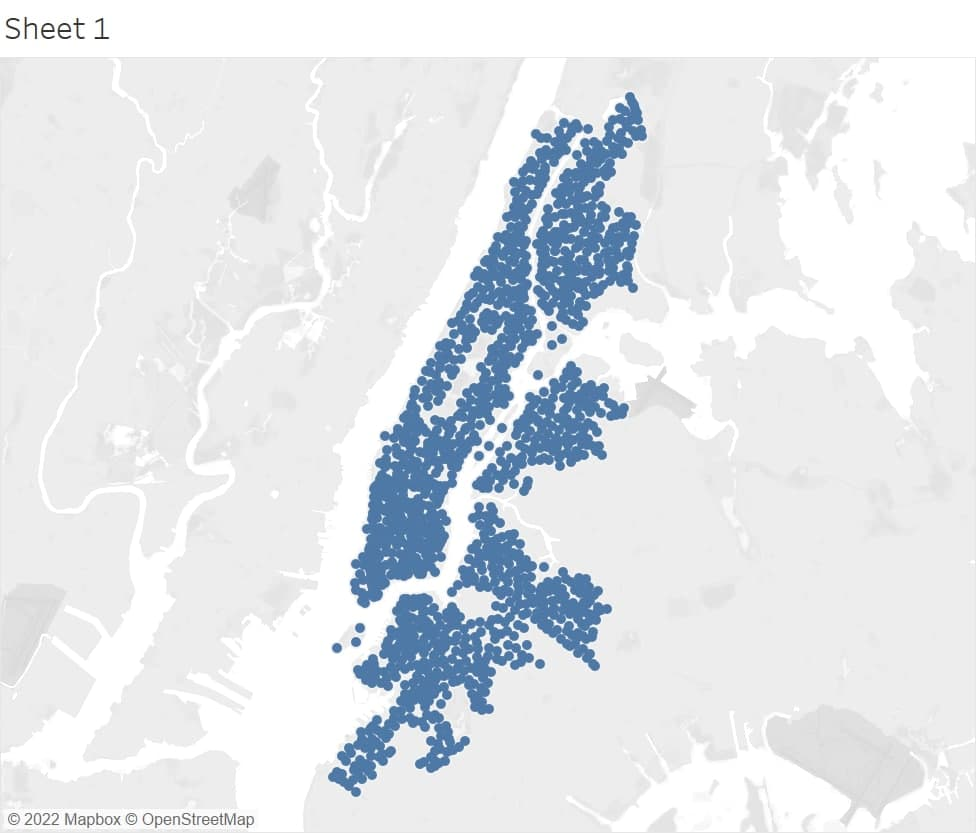
\includegraphics[scale=0.5]{Images/P1.jpg}
\caption{All the bike stations in New York city}
\label{Graph1}
\end{figure}

\begin{figure}
\centering
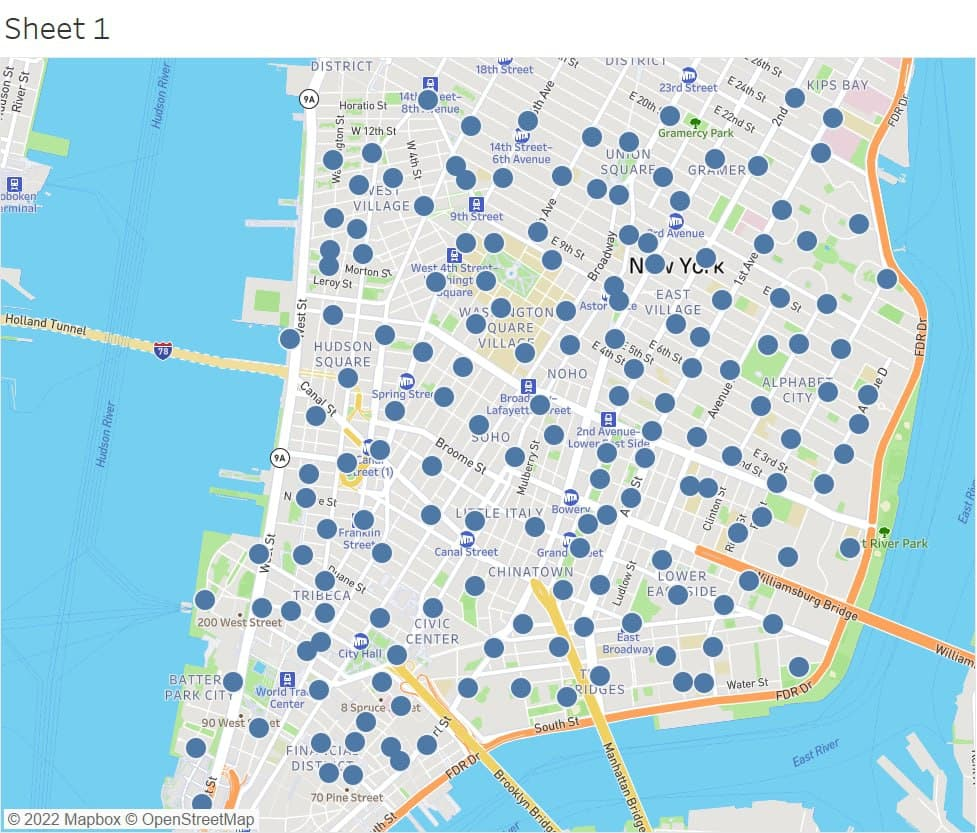
\includegraphics[scale=0.47]{Images/P2.jpg}
\caption{A  map of bike stations located in the south side of Manhattan.}
\label{Graph2}
\end{figure}


\section{Evaluation}


In general, there are two types of evaluation metrics; extrinsic and intrinsic. As for the extrinsic metrics, one can use similar datasets to perform the same analysis. The results of those analyses will determine the extendability of the approaches used. Regarding intrinsic metrics, depending on the task, the data set can be separated into several portions. These separate portions can then be used to examine the generalizability of our approaches. In the case of statistical exams, the same score/result can be expected from different portions of the data set assuming uniform sampling. While some evaluations will need splitting the data, others which are commonly referred to as supervised tasks, such as gender prediction in our case, have their own standard evaluation metrics which will be used accordingly. Not ignoring the viability of quantitative metrics, visualization, as an instance of quantitative metrics, can also be used for assessing the results. In the long run, a collection of all above-mentioned metrics can be aggregated to represent a unified measure to evaluate our results.
 

\bibliographystyle{plain}
\bibliography{references}



\end{document}
\endinput
%%
%% End of file `sample-authordraft.tex'.
